\documentclass{article}[18pt]
\usepackage[utf8]{inputenc}
\usepackage[margin=0.7in]{geometry}
\usepackage{parselines} 
\usepackage{amsmath}
\usepackage{titlesec}
\usepackage{pgfplots}
\usepackage{graphicx}
\usepackage[english]{babel}
\usepackage{fancyhdr}
\usepackage{tikz}
\usetikzlibrary{scopes}
\pgfplotsset{width=10cm,compat=1.9}

\titlespacing\section{0pt}{14pt plus 4pt minus 2pt}{0pt plus 2pt minus 2pt}
\newlength\tindent
\setlength{\tindent}{\parindent}
\setlength{\parindent}{0pt}
\renewcommand{\indent}{\hspace*{\tindent}}

\pagestyle{fancy}
\fancyhf{}
\rhead{Sam Robbins 13SE}
\lhead{A Level Physics - Further Mechanics and Thermal Physics}
\rfoot{Page \thepage}
\pgfdeclarelayer{background layer}
\pgfdeclarelayer{foreground layer}
\pgfsetlayers{background layer,main,foreground layer}

\begin{document}
\begin{center}
\underline{\huge Circular Motion}
\end{center}
\section{Introduction to circular motion}
For an object to be going in a circle a force is needed to accelerate the object. This is because in a circle an object is constantly changing velocity, even if it isn't changing speed.\\
Centripetal force is not an extra force, it is just the name for a resultant force.\\
For an object to be deflected towards the centre, there needs to be a force acting towards the centre.
\subsection{Definitions}
\begin{tabular}{|c|c|c|c|}
\hline
Quantity&Symbol&Unit&Definition\\
\hline
Period&T&Seconds,s&The time taken for an object to complete one revolution\\
\hline
Frequency&f&Hertz,hz&The number of revolutions per second\\
\hline
Angular velocity&$\omega$&$\textrm{rads}^{-1}$&The rate of change in angle(the angle covered per second)\\
\hline
\end{tabular}
\subsection{Formula not on formula book}
$$\omega=\frac{\Delta\theta}{\Delta t}$$
$$a=\frac{\Delta V}{\Delta t}$$
Don't forget application of  $F=ma$ with the equations for force
\section{Circular motion for going over a hump}
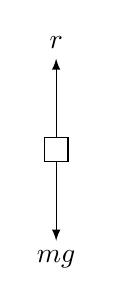
\begin{tikzpicture}[
    force/.style={>=latex,draw=black,fill=black},
    m/.style={rectangle,draw=black,fill=white,minimum size=0.3cm,thin},
]
    \node[m] (m) {};
    {[force,->]
        \draw (m.north) -- ++(0,1) node[above] {$r$};
        \draw (m.south) -- ++(0,-1) node[below] {$mg$};
    }
\end{tikzpicture}
\\
For an object going over a hump the force of the weight is in the opposite direction to the reaction force.\\
The object will leave the ground if $mg>r$.
\subsection{Calculations}
$$F_c=mg-R=\frac{mv^2}{r}$$
\textbf{Calculating the speed at which the car will leave the ground (R=0)}\\
$$mg=\frac{mv_0^2}{r} \qquad V_0=\sqrt{gr}$$
Once the car has left the ground, use SUVAT equations rather than circular motion.
\section{Roundabouts}
On a roundabout the centripetal force is provided by friction.\\
$$F_r=\frac{mv_0^2}{r}$$
To avoid slipping, the centripetal force must be less than the maximum possible for the car and road surface.\\
\textbf{Example question}
\textit{The maximum possible force of friction between a car and the road is 800N, given a mass of 1000kg and a radius of 5m, what is the maximum speed the car can go without slipping}
\newpage
\section{Banked motion}
N is the reaction force\\
$n\sin\theta=\dfrac{mv^2}{r}$ - Force towards the centre of notion is equal to the centripetal force\\
$N\cos\theta=mg$ - The force vertically downwards is equal to the weight\\
$\tan\theta=\dfrac{v^2}{rg}$ - Combining the equations\\
$v^2=gr\tan\theta$ - Re-write
\section{Forces in a circle}
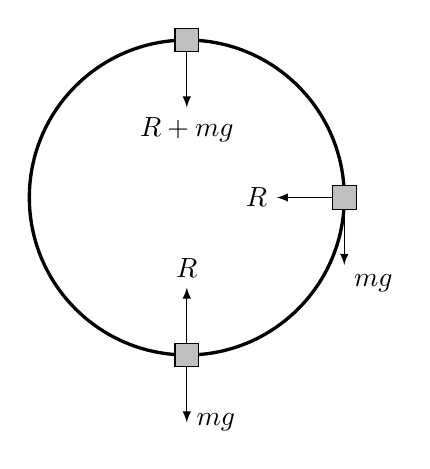
\begin{tikzpicture}[
    force/.style={>=latex,draw=black,fill=black},
    m/.style={rectangle,draw=black,fill=lightgray,minimum size=0.3cm,thin},
]
    \node[m] (m) at (0,-2) {};
    \node[m] (m2) at (0,2) {};
    \node[m] (m3) at (2,0) {};
    {[force,->]
        \draw (m.north) -- ++(0,0.7) node[above] {$R$};
        \draw (m.south) -- ++(0,-0.7) node[right] {$mg$};
    }
    {[force,->]
        \draw (m2.south) -- ++(0,-0.7) node[below] {$R+mg$};
    }
    {[force,->]
        \draw (m3.west) -- ++(-0.7,0) node[left] {$R$};
        \draw (m3.south) -- ++(0,-0.7) node[below right] {$mg$};
    }

\begin{pgfonlayer}{background layer}
    \draw[color=black, very thick](0,0) circle (2);
    \end{pgfonlayer}{background layer}
\end{tikzpicture}
\\
Top: Centripetal force = $R+W$\\
Side: Centripetal force = $R$\\
Bottom: Centripetal force = $R-W$\\
At the top of the loop r=0\\
$v=\sqrt{gr}$





\end{document}